\pdfoutput=1
\documentclass[11pt,a4paper]{article}

% ---------------------------------------------------------------------------
% Localization of D-instability in star interconnections and a sharp bound on
% synchronized groups.
% Author metadata: set the three macros below before submission.
% ---------------------------------------------------------------------------
\newcommand{\PaperAuthor}{}
\newcommand{\PaperAffiliation}{}
\newcommand{\PaperDate}{September 2026}

\usepackage[T1]{fontenc}
\usepackage[utf8]{inputenc}
\usepackage{lmodern}
% Font expansion is off: with it, pdfTeX (MiKTeX) once placed a line far off the page.
\usepackage[expansion=false]{microtype}
\usepackage[a4paper,margin=1.05in]{geometry}
\usepackage{amsmath,amssymb,amsthm,mathtools}
\usepackage{booktabs}
\usepackage{array}
\usepackage{enumitem}
\usepackage{graphicx}
\usepackage{caption}
\captionsetup{font=small}
\captionsetup[table]{justification=raggedright,singlelinecheck=false}
\usepackage{xcolor}
\usepackage[hyphens,obeyspaces,spaces]{url}
\usepackage[colorlinks=true,linkcolor=blue!55!black,citecolor=blue!55!black,urlcolor=blue!55!black]{hyperref}
\hypersetup{pdftitle={Localization of D-instability in star interconnections and a sharp bound on synchronized groups},
  pdfauthor={\PaperAuthor},
  pdfsubject={D-stability, time scales, model reduction},
  pdfkeywords={D-stability, diagonal scaling, time scales, quasi-steady-state approximation, lumping, secant condition, Hurwitz theorem, Lean 4}}

\setlist{itemsep=2pt,topsep=3pt}
\setlength{\emergencystretch}{1.5em}

\theoremstyle{plain}
\newtheorem{theorem}{Theorem}[section]
\newtheorem{proposition}[theorem]{Proposition}
\newtheorem{lemma}[theorem]{Lemma}
\newtheorem{corollary}[theorem]{Corollary}
\theoremstyle{definition}
\newtheorem{definition}[theorem]{Definition}
\newtheorem{example}[theorem]{Example}
\theoremstyle{remark}
\newtheorem{remark}[theorem]{Remark}

\newcommand{\R}{\mathbb{R}}
\newcommand{\C}{\mathbb{C}}
\newcommand{\Real}{\operatorname{Re}}
\newcommand{\Imag}{\operatorname{Im}}
\newcommand{\diag}{\operatorname{diag}}
\newcommand{\Bd}{\operatorname{Bd}}
\newcommand{\val}{\operatorname{val}}
\newcommand{\Cyc}{\operatorname{Cyc}}
\newcommand{\ch}{\operatorname{ch}}
\newcommand{\be}{\mathbf{e}}
\newcommand{\rF}{\mathsf{F}}
\newcommand{\rS}{\mathsf{S}}
\newcommand{\rD}{\mathsf{D}}
\newcommand{\T}{\mathsf{T}}
\DeclareUrlCommand\lean{\urlstyle{tt}}
\def\UrlBreaks{\do\.\do\/\do\-}

\title{Localization of D-instability in star interconnections and a sharp bound on synchronized groups}
\author{\PaperAuthor\\[2pt]\small\PaperAffiliation}
\date{\PaperDate}

\begin{document}
\maketitle

\begin{abstract}
A real square matrix $A$ is D-stable if $AD$ is Hurwitz for every positive diagonal
matrix $D$, that is, if the linear system it describes is stable whatever the positive
time scales of its coordinates. We study star interconnections: a core matrix
$B\in\R^{n\times n}$ together with first-order attachments that read the core through
rank-one interfaces $u_cv_c^\T$, grouped into $k$ channels, with nonzero feedback loads of
either sign. Assigning each attachment to be fast (quasi-steady), slow (frozen), or a member
of a single synchronized group of its channel defines a \emph{boundary system}: a star of
dimension $n+k$ with at most one dynamic lump per channel. We prove that every eigenvalue in
the closed right half-plane of every positive scaling of the star is the same eigenvalue of a
positive scaling of one of its boundary systems. No hypothesis on the core is needed.
Conversely, strict instability of a boundary system lifts to the star. Hence the star is
D-semistable exactly when all its boundary systems are, and it is D-stable if all its
boundary systems are; an explicit example shows that the last implication cannot be
reversed. Both features of the boundary systems are necessary. For every $k\ge2$ a cyclic
star built on the secant condition is not D-stable, while every boundary system with fewer
than $k$ synchronized groups is; and already for one channel, two pieces may have to be
lumped into one synchronized group. The proof combines a compact parametrization of each
attachment's frequency response at a fixed eigenvalue, an exact identity showing that two
attachments of one channel have independent tangents unless their time constants agree, and
an exit argument phrased as a maximum over a compact cube. The theorems, propositions and
lemmas are formally verified in Lean~4 with Mathlib.
\end{abstract}

\noindent\textbf{Keywords:} D-stability; diagonal scaling; time scales;
quasi-steady-state approximation; lumping; model reduction; secant condition; formal
verification.\\[2pt]
\textbf{MSC 2020:} 15A18, 93D09 (primary); 34D20, 93C15 (secondary).

\tableofcontents

% =========================================================================
\section{Introduction}\label{sec:intro}

A real $N\times N$ matrix $A$ is \emph{D-stable} if $AD$ has all its eigenvalues in the
open left half-plane for every positive diagonal matrix $D$~\cite{enthoven1956,arrow1958}.
Writing $T=D^{-1}$, the eigenvalues of $AD$ are the roots of $\det(zT-A)$, the
characteristic values of the system $T\dot x=Ax$ in which coordinate $i$ has time constant
$T_{ii}$. D-stability is therefore stability for all positive time scales, a natural
requirement whenever capacities, volumes or turnover rates are uncertain; see the
surveys~\cite{hershkowitz1992,kushel2019}.

In applications such systems are rarely analysed at full size. One eliminates fast species
by a quasi-steady-state approximation, freezes slow ones~\cite{segel1989,kokotovic1999},
and lumps species with a common time constant into one pool~\cite{wei1969}. The first two
operations are limits in the space of time scales; the third restricts to a diagonal of it.
Stability of a reduced model says nothing, in general, about the full family: a quasi-steady
reduction can lose an oscillation that the full model has~\cite{flach2006,kimtyson2020}.
This paper asks which reduced models decide D-stability, and how many time scales a reduced
model must retain, for a class of interconnections in which the question has a sharp answer.

\paragraph{Stars.} A \emph{star}\footnote{The name refers to the interconnection pattern of
a core with attachments; it is unrelated to star graphs and star sign patterns in
combinatorial matrix theory.} consists of a core $B\in\R^{n\times n}$ and $m$ first-order
attachments (\emph{pieces}). Piece $p$ belongs to a channel $\ch(p)$ among $k$ channels.
Channel $c$ reads the core through $v_c^\T x$ and feeds back along $u_c$, with
$u_c,v_c\in\R^n$. Piece $p$ has a nonzero load $r_p$ of either sign:
\[
  \dot x = Bx+\sum_p r_p\,u_{\ch(p)}w_p,\qquad \dot w_p = v_{\ch(p)}^\T x-w_p ,
\]
with all coordinates then given arbitrary positive time constants. Binding sites, decoys
and buffers acting on one species are coordinate channels, $u_c=v_c=\be_i$; a complex
formed from several species, or a sensor reading a weighted sum, gives a general rank-one
channel.

\paragraph{Boundary systems.} A \emph{boundary choice} sends every piece to $\rF$ (fast,
quasi-steady: it becomes the static load $r_pu_{\ch(p)}v_{\ch(p)}^\T$ of the core),
$\rS$ (slow, frozen: it disappears), or $\rD$ (it joins the synchronized group of its
channel, whose pieces share one time constant and act as a single lumped pool). The
resulting \emph{boundary system} is again a star, with at most one dynamic lump per
channel (Definition~\ref{def:boundary}). It is the reduced model obtained by quasi-steady
elimination, freezing, and lumping within a channel.

\paragraph{Results.} We prove the following, for arbitrary cores, arbitrary rank-one
interfaces and nonzero loads of either sign.
\begin{enumerate}[label=(\Alph*)]
  \item \emph{Spectral localization} (Theorem~\ref{thm:localization}). If some positive
    scaling of the star has an eigenvalue $z$ with $\Real z\ge0$, then some positive
    scaling of some boundary system has the same eigenvalue $z$. No stability hypothesis
    on the core is used.
  \item \emph{Lifting} (Theorem~\ref{thm:lifting}). If some scaling of a boundary system
    has an eigenvalue with positive real part, so does some scaling of the star.
  \item \emph{Criterion} (Corollary~\ref{cor:criterion}). The star is D-semistable if and
    only if all its boundary systems are. It is D-stable if all its boundary systems are,
    and Proposition~\ref{prop:gap} shows that this implication is not an equivalence.
  \item \emph{Sharpness} (Theorem~\ref{thm:sharpness} and Proposition~\ref{prop:lumping}).
    For every $k\ge2$ there is a $k$-channel star that is not D-stable although every
    boundary system with fewer than $k$ synchronized groups is D-stable. For $k=1$ there is
    a star with two pieces that is not D-stable although every boundary system in which at
    most one piece is dynamic is D-stable. So neither the number of groups nor their size
    can be reduced in general.
\end{enumerate}
In modelling terms: for star interconnections, screening stability under all time scales
by reduced models is exact for D-semistability, provided one checks every combination of
quasi-steady, frozen and lumped pieces with one lumped pool per interface; and one can do
neither with fewer lumped pools nor with unlumped pieces. The number of boundary choices is
exponential in the number of pieces. Some such growth is to be expected: for binary-encoded
loads, deciding D-stability is coNP-hard already for stars with one coordinate channel and a
$4\times4$ core whose entries depend on the instance~\cite{companionHard2026}.

\paragraph{Ideas of the proof.} Eliminating the pieces at an eigenvalue $z$ with
$\Real z\ge0$ leaves an $n\times n$ pencil whose determinant is affine in the value
$\ell_c$ of each channel (Lemmas~\ref{lem:elimination} and~\ref{lem:affine}). For non-real
$z$, the value $r_p/(1+zt_p)$ of one piece runs over an arc as its time constant $t_p$ runs
over $(0,\infty)$. We parametrize this arc by $s\in[0,1]$, with $s=0$ the quasi-steady end
and $s=1$ the frozen end, so that the configuration space becomes the compact cube
$[0,1]^P$. An exact identity (Lemma~\ref{lem:sync}) shows that two pieces of one channel move
the channel value in independent directions unless their parameters agree. We then dilate
the core time constants, which pushes the contact out to a maximal dilation over the compact
set of contacts; at the maximum, openness forbids two unequal interior parameters in the
channel, so the channel is of boundary type (Lemma~\ref{lem:exit}). Treating the channels
one by one gives Theorem~\ref{thm:localization} for non-real $z$; real eigenvalues are
handled by an explicit sign-class construction. Lifting is Hurwitz's theorem on zeros of
uniform limits. Sharpness uses the secant condition~\cite{tyson1978,thron1991,arcak2006}: a
fast channel removes one stage from a negative feedback cycle, a slow channel cuts it, and
the thresholds $\sec^N(\pi/N)$ decrease strictly in $N$.

\paragraph{Related work.} Johnson~\cite{johnson1975} characterized D-stability of a stable
matrix by the nonsingularity of $A\pm iD$, and Kushel~\cite{kushel2026} expands
$\det(A+iD)$ recursively, eliminating one scaling variable at a time; this is exact at the
first step and a hierarchy of sufficient tests beyond. Our elimination removes whole
attachment modules instead, and the reduced dimension $n+k$ does not grow with the number
of pieces. Hartfiel~\cite{hartfiel1980} and Cain~\cite{cain1984} characterized the
interior of the set of D-stable matrices (robust D-stability) by D-stability of matrices
built from principal submatrices of $A$ and of their inverses; see the
survey~\cite{kushel2019}. In time-scale language these are limits in which coordinates of
$A$ become frozen or quasi-static. Boundary systems take such limits only on the
attachments, and they keep dynamic lumped pools, which Theorem~\ref{thm:sharpness} and
Proposition~\ref{prop:lumping} show to be indispensable. The link between D-stability and
many small time constants goes back to Khalil and Kokotovi\'c~\cite{khalil1979},
Abed~\cite{abed1986tac,abed1986}, and Abed and Tits~\cite{abedtits1986}: there
D-stability of a fast block is a sufficient condition for stability under asymptotically
small parasitic time constants, whereas here all time scales in $(0,\infty)$ are free and
the localization is exact. Berman and Hershkowitz~\cite{berman1984} characterized acyclic
D-stable matrices, and Simpson-Porco and Monshizadeh~\cite{simpsonporco2022} characterized
diagonal stability of systems with rank-one interconnections. For a single negative
feedback cycle, the secant condition~\cite{tyson1978,thron1991,sontag2006,arcak2006} gives
stability for all time constants below the threshold $\sec^N(\pi/N)$ and instability at
equal time constants above it; Blanchini, Cuba Samaniego, Franco and
Giordano~\cite{blanchini2018} observed that equal time constants are extremal and that a
sufficiently slow element stabilizes a loop. Our sharpness constructions read these facts
through boundary systems. Vertex results for multiaffine families on bounded
boxes~\cite{blanchini2022} have a similar flavour: Theorem~\ref{thm:localization} shows
that, for the piece time constants, it suffices to consider configurations in which the
pieces of each channel take only the values $0$, $\infty$ and one common finite value,
while the core time constants remain free. Inheritance results for reaction
networks~\cite{banaji2018,vassena2024} transfer instability upward, as in
Theorem~\ref{thm:lifting}; to our knowledge the downward direction,
Theorem~\ref{thm:localization}, has no counterpart there. For one coordinate channel with
positive loads and a D-stable core, a companion paper~\cite{companionI2026} gives an exact
test by the boundary systems with at most one dynamic piece, in which the purely static
system enters only through the sign of its determinant; the present results hold for any
core, any interfaces, any signs and any number of channels.

\paragraph{Formal verification.} Every theorem, proposition, corollary and lemma of this
paper is formally verified in Lean~4~\cite{demoura2021} with Mathlib~\cite{mathlib2020}, as
stated; Section~\ref{sec:lean} lists the declarations. The proofs below follow the formal
ones.

\paragraph{Organization.} Section~\ref{sec:setting} fixes notation and states the results.
Section~\ref{sec:elimination} eliminates the pieces. Section~\ref{sec:channel} studies one
channel at a fixed eigenvalue, and Section~\ref{sec:exit} proves localization of non-real
eigenvalues. Section~\ref{sec:proofs} treats real eigenvalues and proves lifting, the
criterion and Proposition~\ref{prop:gap}. Section~\ref{sec:sharpness} proves the
sharpness results. Section~\ref{sec:discussion} discusses scope and open problems, and
Section~\ref{sec:lean} the formalization.

% =========================================================================
\section{Setting and main results}\label{sec:setting}

\subsection{D-stability}

Let $A\in\R^{N\times N}$. For a vector $d\in(0,\infty)^N$ write $AD=A\diag(d)$, a
\emph{positive scaling} of $A$. We say that $A$ is
\begin{itemize}
  \item \emph{D-stable} if every positive scaling of $A$ has all eigenvalues in
    $\{\Real z<0\}$;
  \item \emph{D-semistable} if no positive scaling of $A$ has an eigenvalue in
    $\{\Real z>0\}$;
  \item \emph{D-unstable} if it is not D-semistable, and \emph{marginal} if it is
    D-semistable but not D-stable, that is, some positive scaling has an eigenvalue on the
    imaginary axis (possibly $0$) and none has one in $\{\Real z>0\}$.
\end{itemize}
Since $AD$ and $DA$ are similar, the side on which one scales does not matter. With
$T=\diag(d)^{-1}$, the \emph{time constants}, a number $z$ is an eigenvalue of $AD$ if and
only if $\det(zT-A)=0$.

\subsection{Stars and boundary systems}

\begin{definition}[Star]\label{def:star}
Let $B\in\R^{n\times n}$, let $C$ be a finite set of $k$ \emph{channels} with vectors
$u_c,v_c\in\R^n$, and let $P$ be a finite set of $m$ \emph{pieces} with a channel map
$\ch\colon P\to C$ and loads $r\in\R^P$. The \emph{star}
$A=\operatorname{star}(B,u,v,\ch,r)\in\R^{(n+m)\times(n+m)}$ is
\[
  A=\begin{pmatrix} B & U\\ V & -I_m\end{pmatrix},
  \qquad U\be_p=r_p\,u_{\ch(p)},\qquad \be_p^\T V=v_{\ch(p)}^\T .
\]
\end{definition}

Throughout, the time constants of a positive scaling of a star are written
$T=\diag(q,t)$ with $q\in(0,\infty)^n$ (core) and $t\in(0,\infty)^P$ (pieces), and
$Q=\diag(q)$. For $z\in\C$ with $1+zt_p\ne0$ for all $p$, the \emph{channel values} and
the \emph{reduced pencil} are
\begin{equation}\label{eq:pencil}
  \ell_c(z)=\sum_{\ch(p)=c}\frac{r_p}{1+zt_p},\qquad
  M_q(\ell)=zQ-B-\sum_{c\in C}\ell_c\,u_cv_c^\T .
\end{equation}

\begin{definition}[Boundary systems]\label{def:boundary}
A \emph{boundary choice} is a map $\sigma\colon P\to\{\rF,\rS,\rD\}$. Its
\emph{boundary system} is the star with one piece per channel
\[
  \Bd_\sigma=\operatorname{star}\bigl(B_\sigma,u,v,\mathrm{id}_C,R^\sigma\bigr),\qquad
  B_\sigma=B+\sum_{\sigma(p)=\rF}r_p\,u_{\ch(p)}v_{\ch(p)}^\T,\qquad
  R^\sigma_c=\sum_{\ch(p)=c,\ \sigma(p)=\rD}r_p ,
\]
of dimension $n+k$. The \emph{synchronized group} of channel $c$ is
$\{p:\ch(p)=c,\ \sigma(p)=\rD\}$, and the number of synchronized groups of $\sigma$ is the
number of channels whose group is nonempty.
\end{definition}

The scaling of a boundary system is $\diag(d)$ with entries $d_c$ on the lump coordinates,
and its time constants are written $(q,\tau)$, $\tau\in(0,\infty)^C$. The lump of a channel
whose group is empty carries load $0$; the matrix is then block triangular, and the lump
only contributes the eigenvalue $-d_c$. A boundary system thus has at most one dynamic lump
per channel. Its reduced pencil is $zQ-B_\sigma-\sum_cR^\sigma_c(1+z\tau_c)^{-1}u_cv_c^\T$.
For $z\ne0$ with $\Real z\ge0$ this is the limit of the pencil~\eqref{eq:pencil} of the star
as the time constants of $\rF$-pieces tend to $0$ and those of $\rS$-pieces tend to
$\infty$, with the pieces of the group of channel $c$ all at time constant $\tau_c$. Lumping
is exact within a channel because its pieces share $u_c$ and $v_c$. Table~\ref{tab:dictionary}
records the modelling reading; it is interpretation only and is not used in the proofs.

\begin{table}[tb]
\centering\small
\caption{Modelling reading of the objects (interpretation only).}\label{tab:dictionary}
\begin{tabular}{@{}p{0.34\linewidth}p{0.58\linewidth}@{}}
\toprule
Object & Reading\\
\midrule
positive scaling $AD$ & a choice of positive time constants $T=D^{-1}$ (capacities, volumes, turnover)\\
coordinate channel $u_c=v_c=\be_i$ & attachments binding and releasing one species (sites, decoys, buffers)\\
general rank-one channel & an attachment driven by $v_c^\T x$ and acting along $u_c$ (a complex, a sensor)\\
piece role $\rF$ & quasi-steady-state approximation of that piece\\
piece role $\rS$ & the piece is frozen on the time scale of interest\\
synchronized group $\rD$ & pieces of one channel with a common time constant, lumped into one pool\\
boundary system $\Bd_\sigma$ & one reduced model obtained by these operations (possibly at other core time constants than the full model)\\
\bottomrule
\end{tabular}
\end{table}

Pieces of load $0$ do not act on the core: deleting them only removes eigenvalues $-d_p$.
The assumption of nonzero loads below is therefore a normalization.

\subsection{Main results}

\begin{theorem}[Spectral localization]\label{thm:localization}
Let $A$ be a star with all loads nonzero, let $z\in\C$ with $\Real z\ge0$, and suppose
that $z$ is an eigenvalue of some positive scaling of $A$. Then there is a boundary choice
$\sigma$ such that $z$ is an eigenvalue of some positive scaling of $\Bd_\sigma$.
\end{theorem}

\begin{theorem}[Lifting]\label{thm:lifting}
Let $A$ be a star. If some positive scaling of some boundary system $\Bd_\sigma$ has an
eigenvalue with positive real part, then some positive scaling of $A$ has an eigenvalue
with positive real part.
\end{theorem}

\begin{corollary}[Criterion]\label{cor:criterion}
Let $A$ be a star with all loads nonzero.
\begin{enumerate}[label=(\alph*)]
  \item If every boundary system $\Bd_\sigma$ is D-stable, then $A$ is D-stable.
  \item $A$ is D-semistable if and only if every boundary system $\Bd_\sigma$ is
    D-semistable. Equivalently, $A$ is D-unstable if and only if some $\Bd_\sigma$ is.
\end{enumerate}
\end{corollary}

\begin{proposition}[The criterion is not an equivalence]\label{prop:gap}
Let $n=2$, one channel with $u=v=\be_1$, and one piece of load $1$, so that
\[
  B=\begin{pmatrix}-1&-1\\1&0\end{pmatrix},\qquad
  A=\begin{pmatrix}-1&-1&1\\1&0&0\\1&0&-1\end{pmatrix}.
\]
The star $A$ is D-stable, but its boundary system with the piece fast has the eigenvalue
$i$ at unit time constants.
\end{proposition}

For sharpness we use two examples. The first is cyclic. For $k\ge2$ index the channels by
$\mathbb{Z}/k$ and let $\Cyc_k(\rho)$, $\rho>0$, be the star with core $-I_k$, one piece of
load $\rho$ in every channel, $v_c=\be_{c+1}$, $u_c=\be_c$ for $c\ne k-1$, and
$u_{k-1}=-\be_{k-1}$. Its graph is a single negative feedback cycle through $2k$
first-order stages, $x_0\leftarrow w_0\leftarrow x_1\leftarrow w_1\leftarrow\cdots\leftarrow
w_{k-1}\leftarrow x_0$, with loop gain $g=\rho^k$.

\begin{theorem}[Sharpness of the number of groups]\label{thm:sharpness}
Let $k\ge2$ and $\rho>0$ with
\begin{equation}\label{eq:window}
  \rho\cos^2\!\Bigl(\frac{\pi}{2k}\Bigr)>1
  \qquad\text{and}\qquad
  \rho^k\cos^{2k-1}\!\Bigl(\frac{\pi}{2k-1}\Bigr)<1 .
\end{equation}
Then at unit time constants $\Cyc_k(\rho)$ has the eigenvalue $\sqrt\rho\,e^{i\pi/2k}-1$,
whose real part is positive; in particular $\Cyc_k(\rho)$ is D-unstable. Every boundary
system of $\Cyc_k(\rho)$ with fewer than $k$ synchronized groups is D-stable. For every
$k\ge2$ some $\rho$ satisfies~\eqref{eq:window}.
\end{theorem}

Since both conditions in~\eqref{eq:window} are monotone in $\rho$, the admissible $\rho$
form an open interval. In terms of the loop gain, \eqref{eq:window} reads
$\sec^{2k}(\pi/2k)<g<\sec^{2k-1}(\pi/(2k-1))$; for $k=2$ this is $4<g<8$
(Example~\ref{ex:cyc2}, Figure~\ref{fig:secant}). In $\Cyc_k$ every channel carries one
piece, so Theorem~\ref{thm:sharpness} concerns the number of dynamic channels. The second
example shows that lumping several pieces is also necessary.

\begin{proposition}[Synchronization is needed]\label{prop:lumping}
Let $n=2$, one channel with $v=\be_2$ and $u=-\be_1$, and two pieces of load $125/16$
each, on the core
\[
  B=\begin{pmatrix}-1&0\\1&-1\end{pmatrix}.
\]
At unit time constants the star has the
eigenvalue $-1+\tfrac52e^{i\pi/3}=\tfrac14+\tfrac{5\sqrt3}{4}i$; in particular it is
D-unstable. Every boundary system in which at most one piece is synchronized is D-stable.
\end{proposition}

The star of Proposition~\ref{prop:lumping} is a negative feedback loop
$x_1\to x_2\to\{w_1,w_2\}\dashv x_1$ of total gain $125/8$. Each pool alone carries half the
gain, below the three-stage threshold $\sec^3(\pi/3)=8$, and a quasi-steady pool only adds
static feedback; only the two pools lumped together destabilize.

\begin{remark}[Scope of the statements]\label{rem:scope}
We record three features of the statements.
\begin{enumerate}[label=(\roman*)]
  \item Theorem~\ref{thm:localization} holds for $z=0$ with $\sigma\equiv\rF$, and for
    real $z>0$ with a boundary choice that has no fast pieces
    (Lemmas~\ref{lem:zero} and~\ref{lem:real}); in both cases the same core time constants
    can be kept.
  \item Corollary~\ref{cor:criterion}(a) asks for D-stability of every boundary system,
    including the purely static ones, $\Bd_{\sigma\equiv\rF}$ and $\Bd_{\sigma\equiv\rS}$
    (whose core is $B$). Proposition~\ref{prop:gap} shows that a boundary system can be
    marginal while the star is D-stable: the limits $t_p\to0$ and $t_p\to\infty$ are not
    attained.
  \item $\Bd_\sigma$ depends on $\sigma$ only through the pairs
    $\bigl(\sum_{\ch(p)=c,\sigma(p)=\rF}r_p,\ R^\sigma_c\bigr)$, $c\in C$, of fast and
    synchronized load sums. Distinct boundary choices therefore often give the same boundary
    system; when all loads of a channel are equal, only the numbers of its fast and
    synchronized pieces matter.
\end{enumerate}
\end{remark}

% =========================================================================
\section{Elimination of the pieces}\label{sec:elimination}

\begin{lemma}[Elimination]\label{lem:elimination}
Let $A$ be a star, $q\in(0,\infty)^n$, $t\in(0,\infty)^P$, and $z\in\C$ with $1+zt_p\ne0$
for all $p$. Then $z$ is an eigenvalue of $A\diag(q,t)^{-1}$ if and only if the reduced
pencil $M_q(\ell(z))$ of~\eqref{eq:pencil} is singular.
\end{lemma}

\begin{proof}
An eigenvector of $A\diag(q,t)^{-1}$ for $z$ is $\diag(q,t)(x,w)$ with $(x,w)\ne0$ and
$(zT-A)(x,w)=0$, $T=\diag(q,t)$. The row of piece $p$ reads $zt_pw_p=v_{\ch(p)}^\T x-w_p$,
so $w_p=v_{\ch(p)}^\T x/(1+zt_p)$. Substituting into the core rows
$zQx=Bx+\sum_pr_pu_{\ch(p)}w_p$ and grouping the pieces by channel gives $M_q(\ell(z))x=0$.
If $x=0$ then $w=0$, so $x\ne0$. Conversely, a nonzero kernel vector $x$ of
$M_q(\ell(z))$ and $w_p=v_{\ch(p)}^\T x/(1+zt_p)$ satisfy $(zT-A)(x,w)=0$.
\end{proof}

\begin{lemma}[Rank-one updates are affine]\label{lem:affine}
For $M\in\C^{n\times n}$, $u,v\in\C^n$ and $\lambda\in\C$,
\[
  \det\bigl(M-\lambda\,uv^\T\bigr)=\det M+\lambda\,\beta(M,u,v),\qquad
  \beta(M,u,v)=\det\begin{pmatrix}M&u\\ v^\T&0\end{pmatrix}.
\]
\end{lemma}

\begin{proof}
By the Schur complement of the unit $(2,2)$ entry,
$\det(M-\lambda uv^\T)=\det\begin{pmatrix}M&u\\ \lambda v^\T&1\end{pmatrix}$. The last row
is $\lambda(v^\T,0)+(0,1)$, and the determinant is linear in it.
\end{proof}

In particular, for fixed $z$ and $q$, $\det M_q(\ell)$ is affine in each channel value
$\ell_c$ separately. No invertibility of $zQ-B$ is needed.

\begin{lemma}[Diagonal dominance]\label{lem:dilation}
Let $q\in(0,\infty)^n$, $K\ge0$ and
$h_i=\sum_j\bigl(|B_{ij}|+K\sum_c|u_{c,i}||v_{c,j}|\bigr)$. If $z\in\C$ satisfies
$|z|q_i>h_i$ for every $i$, then $M_q(\ell)$ is nonsingular whenever $|\ell_c|\le K$ for all
$c$. In particular, for $z\ne0$ and $\kappa\ge\kappa_0=1+\sum_ih_i/(|z|q_i)$, the matrix
$M_{\kappa q}(\ell)$ is nonsingular whenever $|\ell_c|\le K$ for all $c$.
\end{lemma}

\begin{proof}
Put $E=B+\sum_c\ell_cu_cv_c^\T$, so that $\sum_j|E_{ij}|\le h_i$ and $M_q(\ell)=zQ-E$.
If $|z|q_i>h_i$ for every $i$, the matrix $zQ-E$ is strictly diagonally dominant by rows,
hence nonsingular by the Lévy--Desplanques theorem~\cite{taussky1949}. For the dilation,
$|z|\kappa q_i\ge|z|\kappa_0q_i>h_i$.
\end{proof}

% =========================================================================
\section{One channel at a fixed eigenvalue}\label{sec:channel}

Throughout this section and the next, $z\in\C$ is fixed with
\[
  \Real z\ge0\qquad\text{and}\qquad \Imag z\ne0 .
\]
For $s\in\R$ put $\alpha(s)=1-s+sz$ and
\[
  \val_z(s)=\frac{1-s}{1-s+sz}.
\]
The denominator never vanishes: $\Imag\alpha(s)=s\Imag z$ vanishes only at $s=0$, where
$\alpha=1$.

\begin{lemma}[Arc parametrization]\label{lem:arc}
The function $\val_z$ has the following properties.
\begin{enumerate}[label=(\alph*)]
  \item $\val_z(0)=1$ and $\val_z(1)=0$.
  \item For $t>0$, $1/(1+zt)=\val_z\bigl(t/(1+t)\bigr)$; for $s\in(0,1)$,
    $\val_z(s)=1/(1+z\,\tfrac{s}{1-s})$.
  \item $|\val_z(s)|\le1$ for $s\in[0,1]$.
  \item $\val_z$ is smooth, with $\val_z'(s)=-z/\alpha(s)^2$.
\end{enumerate}
\end{lemma}

\begin{proof}
(a) and (b) are direct. For (c), $|1-s|=1-s\le1-s+s\Real z=\Real\alpha(s)\le|\alpha(s)|$.
For (d), the quotient rule gives the numerator $-\alpha(s)-(1-s)(z-1)=-z$.
\end{proof}

Thus, as its time constant runs over $[0,\infty]$, a piece of load $r$ contributes to its
channel the points $r\val_z(s)$, $s\in[0,1]$, of an arc from $r$ (the quasi-steady end,
$s=0$) to $0$ (the frozen end, $s=1$); see Figure~\ref{fig:arcs}. The whole configuration
space of the pieces is the compact cube $[0,1]^P$.

\begin{lemma}[Synchronization identity]\label{lem:sync}
For real $r_p,r_{p'},s_p,s_{p'}$ write $\xi(s)=1-s+s\Real z$ and $\eta(s)=s\Imag z$, so that
$\alpha=\xi+i\eta$. Then
\[
  \Imag\Bigl(\overline{r_p\val_z'(s_p)}\;r_{p'}\val_z'(s_{p'})\Bigr)
  =\frac{2\,r_pr_{p'}\,|z|^2\,\Imag z\,\bigl(\xi(s_p)\xi(s_{p'})+\eta(s_p)\eta(s_{p'})\bigr)\,(s_p-s_{p'})}
        {|\alpha(s_p)|^4\,|\alpha(s_{p'})|^4}.
\]
In particular, if $r_pr_{p'}\ne0$ and $s_p,s_{p'}\in(0,1)$ are distinct, then
$r_p\val_z'(s_p)$ and $r_{p'}\val_z'(s_{p'})$ are linearly independent over $\R$, whatever
the signs of $r_p$ and $r_{p'}$.
\end{lemma}

\begin{proof}
Write $\alpha_p=\alpha(s_p)$. By Lemma~\ref{lem:arc}(d),
$\overline{\val_z'(s_p)}\val_z'(s_{p'})=|z|^2\bigl(\alpha_p\overline{\alpha_{p'}}\bigr)^2/
(|\alpha_p|^4|\alpha_{p'}|^4)$. Moreover
$\Real(\alpha_p\overline{\alpha_{p'}})=\xi_p\xi_{p'}+\eta_p\eta_{p'}$ and
$\Imag(\alpha_p\overline{\alpha_{p'}})=\eta_p\xi_{p'}-\xi_p\eta_{p'}=(s_p-s_{p'})\Imag z$,
and $\Imag(w^2)=2\Real w\Imag w$. For the second statement, $\xi(s)\ge1-s>0$ on $(0,1)$ since
$\Real z\ge0$, and $\eta_p\eta_{p'}=s_ps_{p'}(\Imag z)^2\ge0$, so the right-hand side is
nonzero; two complex numbers $w_1,w_2$ are $\R$-independent exactly when
$\Imag(\overline{w_1}w_2)\ne0$.
\end{proof}

\begin{lemma}[Openness]\label{lem:open}
Let $r_p,r_{p'}\ne0$, let $s_p\ne s_{p'}$ lie in $(0,1)$ and let $c_0\in\C$. For the map
$F(x,y)=c_0+r_p\val_z(x)+r_{p'}\val_z(y)$ from $\R^2$ to $\C$, the image of every
neighbourhood of $(s_p,s_{p'})$ is a neighbourhood of $F(s_p,s_{p'})$.
\end{lemma}

\begin{proof}
$F$ is continuously differentiable, and its derivative at $(s_p,s_{p'})$,
$(x,y)\mapsto r_p\val_z'(s_p)x+r_{p'}\val_z'(s_{p'})y$, is an $\R$-linear bijection
$\R^2\to\C$ by Lemma~\ref{lem:sync}. The inverse function theorem applies.
\end{proof}

\begin{figure}[tb]
\centering
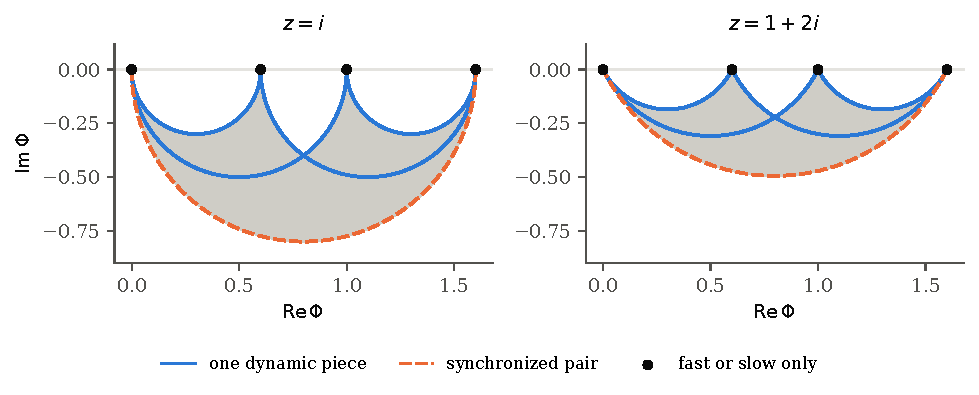
\includegraphics[width=\linewidth]{figures/fig_arcs.pdf}
\caption{One channel at a fixed eigenvalue $z$ (left: $z=i$; right: $z=1+2i$) with two
pieces of loads $r_1=1$ and $r_2=0.6$. Grey: the attainable channel values
$r_1\val_z(s_1)+r_2\val_z(s_2)$, $s\in[0,1]^2$. Coloured: values of boundary-type
configurations, in which the pieces are fast, slow, or share one parameter. By
Lemma~\ref{lem:open}, configurations with two unequal interior parameters give interior
points, so the boundary of the grey region consists of boundary-type values.}
\label{fig:arcs}
\end{figure}

% =========================================================================
\section{The exit lemma and non-real eigenvalues}\label{sec:exit}

Let $A$ be a star with all loads nonzero, and fix $z$ as in Section~\ref{sec:channel}. For
$s\in[0,1]^P$ define the channel values
\[
  \Phi_c(s)=\sum_{\ch(p)=c}r_p\val_z(s_p),\qquad c\in C .
\]
A pair $(q,s)\in(0,\infty)^n\times[0,1]^P$ is a \emph{generalized contact} if
$\det M_q(\Phi(s))=0$. A configuration $s$ is \emph{of boundary type in channel} $c$ if all
its interior parameters in $c$ coincide: $s_p=s_{p'}$ whenever $\ch(p)=\ch(p')=c$ and
$s_p,s_{p'}\in(0,1)$.

\begin{lemma}[Exit lemma]\label{lem:exit}
Let $(q,s)$ be a generalized contact and $c\in C$. There are $\kappa\ge1$ and
$s'\in[0,1]^P$, equal to $s$ outside channel $c$ and of boundary type in channel $c$, such
that $(\kappa q,s')$ is a generalized contact.
\end{lemma}

\begin{proof}
Let $\ell^0$ be $\Phi(s)$ with its $c$-th entry replaced by $0$. For configurations
$\tilde s$ that agree with $s$ outside channel $c$, Lemma~\ref{lem:affine} gives
\[
  \det M_{\kappa q}\bigl(\Phi(\tilde s)\bigr)=a(\kappa)+\Phi_c(\tilde s)\,b(\kappa),\qquad
  a(\kappa)=\det M_{\kappa q}(\ell^0),\quad
  b(\kappa)=\beta\bigl(M_{\kappa q}(\ell^0),u_c,v_c\bigr),
\]
and $a,b$ are polynomials in $\kappa$. Let $K=\sum_p|r_p|$; by Lemma~\ref{lem:arc}(c)
every channel value of every configuration has modulus at most $K$, so
Lemma~\ref{lem:dilation} provides $\kappa_0$ such that no generalized contact of this form
exists at dilations $\kappa\ge\kappa_0$. The function $\val_z$ is continuous, so the set
\[
  \mathcal S=\bigl\{(\kappa,\tilde s)\in[1,\kappa_0]\times[0,1]^P:\ \tilde s=s\text{ outside }c,\
  a(\kappa)+\Phi_c(\tilde s)b(\kappa)=0\bigr\}
\]
is closed in a compact set; it contains $(1,s)$. Let $(\kappa_*,s_*)\in\mathcal S$ maximize
$\kappa$.

If $b(\kappa_*)=0$, then $a(\kappa_*)=0$. The configuration $s'$ equal to $s$ outside $c$
and to $1$ on channel $c$ has $\Phi_c(s')=0$ by Lemma~\ref{lem:arc}(a), so
$(\kappa_*q,s')$ is a generalized contact, and $s'$ is of boundary type in $c$.

If $b(\kappa_*)\ne0$, then $b\ne0$ on a neighbourhood of $\kappa_*$, where
$h(\kappa)=-a(\kappa)/b(\kappa)$ is continuous with $h(\kappa_*)=\Phi_c(s_*)$. Suppose that
$s_*$ is not of boundary type in $c$: some pieces $p\ne p'$ of channel $c$ have parameters
$s_{*p}\ne s_{*p'}$ in $(0,1)$. By Lemma~\ref{lem:open}, the values $\Phi_c(\tilde s)$, where
$\tilde s$ arises from $s_*$ by moving $s_{*p}$ and $s_{*p'}$ inside $(0,1)$, fill a
neighbourhood of $\Phi_c(s_*)$. Hence for some $\kappa_1>\kappa_*$ close to $\kappa_*$ there
is such an $\tilde s$ with $\Phi_c(\tilde s)=h(\kappa_1)$, that is,
$a(\kappa_1)+\Phi_c(\tilde s)b(\kappa_1)=0$. By the choice of $\kappa_0$ we have
$\kappa_1<\kappa_0$, and $\kappa_1>\kappa_*\ge1$, so $(\kappa_1,\tilde s)\in\mathcal S$,
contradicting the maximality of $\kappa_*$. Therefore $s'=s_*$ is of boundary type in $c$,
and $\kappa=\kappa_*$ works.
\end{proof}

\begin{proposition}[Channel induction]\label{prop:induction}
If $(q,s)$ is a generalized contact, there is a generalized contact $(q',s')$ with $s'$ of
boundary type in every channel.
\end{proposition}

\begin{proof}
Apply Lemma~\ref{lem:exit} to the channels one at a time, in any order. Each step changes
only the parameters of its own channel and dilates the core time constants. Being of
boundary type in a channel depends only on that channel's parameters, so the channels
already treated keep the property.
\end{proof}

No stability hypothesis on $B$, or on any matrix met along the way, has been used.

\begin{lemma}[Boundary configurations are boundary systems]\label{lem:boundary}
Let $s\in[0,1]^P$ be of boundary type in every channel. Put $\sigma(p)=\rF$ if $s_p=0$,
$\sigma(p)=\rS$ if $s_p=1$, and $\sigma(p)=\rD$ otherwise. For each channel $c$ whose
group is nonempty let $s^0_c$ be the common interior parameter and
$\tau_c=s^0_c/(1-s^0_c)$; otherwise $\tau_c=1$. Then for every $q$,
\[
  M_q(\Phi(s))=zQ-B_\sigma-\sum_{c}\frac{R^\sigma_c}{1+z\tau_c}\,u_cv_c^\T ,
\]
the reduced pencil of $\Bd_\sigma$ at time constants $(q,\tau)$. Consequently, if $(q,s)$ is
a generalized contact, then $z$ is an eigenvalue of $\Bd_\sigma\diag(q,\tau)^{-1}$.
\end{lemma}

\begin{proof}
By Lemma~\ref{lem:arc}(a),(b), $\Phi_c(s)=\sum_{\ch(p)=c,\sigma(p)=\rF}r_p+
R^\sigma_c/(1+z\tau_c)$, and the fast terms are exactly the static loads in $B_\sigma$.
Since $\Real z\ge0$ and $\tau_c>0$, $1+z\tau_c\ne0$, and Lemma~\ref{lem:elimination},
applied to $\Bd_\sigma$, gives the last statement.
\end{proof}

\begin{proof}[Proof of Theorem~\ref{thm:localization} for non-real $z$]
Let $z$ with $\Real z\ge0$ and $\Imag z\ne0$ be an eigenvalue of
$A\diag(q,t)^{-1}$. Since $\Real z\ge0$, $1+zt_p\ne0$, and Lemma~\ref{lem:elimination}
shows that $M_q(\ell(z))$ is singular. By Lemma~\ref{lem:arc}(b),
$\ell(z)=\Phi(s)$ with $s_p=t_p/(1+t_p)$, so $(q,s)$ is a generalized contact.
Proposition~\ref{prop:induction} and Lemma~\ref{lem:boundary} finish the proof.
\end{proof}

% =========================================================================
\section{Real eigenvalues, lifting and the criterion}\label{sec:proofs}

\begin{lemma}[Zero eigenvalues]\label{lem:zero}
If $0$ is an eigenvalue of $A\diag(q,t)^{-1}$ for a star $A$, then $0$ is an eigenvalue of a
positive scaling of $\Bd_{\sigma\equiv\rF}$ with the same core time constants $q$.
\end{lemma}

\begin{proof}
At $z=0$, $\ell_c(0)=\sum_{\ch(p)=c}r_p$ and $M_q(\ell(0))=-B_{\sigma\equiv\rF}$. The
boundary system $\Bd_{\sigma\equiv\rF}$ has only zero lumps, so its reduced pencil at $z=0$ is
also $-B_{\sigma\equiv\rF}$. Apply Lemma~\ref{lem:elimination} twice.
\end{proof}

\begin{lemma}[Real positive eigenvalues]\label{lem:real}
If a positive scaling $A\diag(q,t)^{-1}$ of a star has a real eigenvalue $z>0$, then there
are a boundary choice $\sigma$ without fast pieces and $\tau\in(0,\infty)^C$ such that $z$ is
an eigenvalue of $\Bd_\sigma\diag(q,\tau)^{-1}$.
\end{lemma}

\begin{proof}
Put $a_p=1/(1+zt_p)\in(0,1)$, so that the channel values
$\ell_c=\ell_c(z)=\sum_{\ch(p)=c}r_pa_p$ are real, and let $G^+_c$ and $G^-_c$ be the sums of
the positive and of the negative loads of channel $c$. If $\ell_c>0$, some load of $c$ is
positive, and $\ell_c\le\sum_{\ch(p)=c,\,r_p>0}r_pa_p<G^+_c$; symmetrically $G^-_c<\ell_c$ if
$\ell_c<0$. Define $\sigma(p)=\rD$ if $\ell_{\ch(p)}\ne0$ and $r_p\ell_{\ch(p)}>0$, and
$\sigma(p)=\rS$ otherwise. Then $B_\sigma=B$, and $R^\sigma_c$ equals $G^+_c$, $G^-_c$ or
$0$ according as $\ell_c$ is positive, negative or zero. Put $\tau_c=(R^\sigma_c/\ell_c-1)/z>0$
if $\ell_c\ne0$ and $\tau_c=1$ otherwise. Then $R^\sigma_c/(1+z\tau_c)=\ell_c$ for every $c$,
so the reduced pencil of $\Bd_\sigma$ at $(q,\tau)$ coincides with $M_q(\ell(z))$, which is
singular by Lemma~\ref{lem:elimination}. Apply Lemma~\ref{lem:elimination} to $\Bd_\sigma$.
\end{proof}

\begin{proof}[Proof of Theorem~\ref{thm:localization}]
The cases $z=0$, $z>0$ and $\Imag z\ne0$ are Lemma~\ref{lem:zero}, Lemma~\ref{lem:real} and
Section~\ref{sec:exit}.
\end{proof}

\begin{proof}[Proof of Theorem~\ref{thm:lifting}]
Let $z_0$, $\Real z_0>0$, be an eigenvalue of $\Bd_\sigma\diag(q,\tau)^{-1}$. For
$\varepsilon\in[0,1]$ and $\Real z>0$ put
\[
  \Delta_\varepsilon(z)=\det\Bigl(zQ-B-\sum_c\ell^\varepsilon_c(z)\,u_cv_c^\T\Bigr),\quad
  \ell^\varepsilon_c(z)=\!\!\sum_{\substack{\ch(p)=c\\ \sigma(p)=\rF}}\!\!\frac{r_p}{1+z\varepsilon}
  +\!\!\sum_{\substack{\ch(p)=c\\ \sigma(p)=\rD}}\!\!\frac{r_p}{1+z\tau_c}
  +\!\!\sum_{\substack{\ch(p)=c\\ \sigma(p)=\rS}}\!\!\frac{r_p\,\varepsilon}{\varepsilon+z}.
\]
For $\varepsilon>0$ this is the reduced determinant~\eqref{eq:pencil} of $A$ at the time
constants $q$ (core), $\varepsilon$ ($\rF$-pieces), $\tau_{\ch(p)}$ ($\rD$-pieces) and
$1/\varepsilon$ ($\rS$-pieces), since $\varepsilon/(\varepsilon+z)=1/(1+z/\varepsilon)$. At
$\varepsilon=0$ it is the reduced determinant of $\Bd_\sigma$ at $(q,\tau)$, so
$\Delta_0(z_0)=0$ by Lemma~\ref{lem:elimination}. All denominators have positive real part,
so $(\varepsilon,z)\mapsto\Delta_\varepsilon(z)$ is continuous on
$[0,1]\times\{\Real z>0\}$ and holomorphic in $z$. Each $|\ell^0_c(z)|\le\sum_p|r_p|$, so by
Lemma~\ref{lem:dilation} $\Delta_0(z)\ne0$ for all large real $z$. Hence the zeros of
$\Delta_0$ in the right half-plane are isolated, and there is $\varrho\in(0,\Real z_0/2)$ such
that $\Delta_0$ has no zero on the circle $|z-z_0|=\varrho$. Let $\delta>0$ be the minimum
of $|\Delta_0|$ on this circle. By uniform continuity on the compact set
$[0,1]\times\{|z-z_0|\le\varrho\}$ there is $\varepsilon\in(0,1]$ with
$|\Delta_\varepsilon-\Delta_0|<\delta/2$ on the closed disc. If $\Delta_\varepsilon$ had no
zero in the closed disc, the maximum modulus principle applied to $1/\Delta_\varepsilon$ would
give $|\Delta_\varepsilon(z_0)|\ge\min_{|z-z_0|=\varrho}|\Delta_\varepsilon|\ge\delta/2$,
whereas $|\Delta_\varepsilon(z_0)|=|\Delta_\varepsilon(z_0)-\Delta_0(z_0)|<\delta/2$. So
$\Delta_\varepsilon(z_1)=0$ for some $z_1$ with $\Real z_1\ge\Real z_0-\varrho>0$, and $z_1$ is
an eigenvalue of the corresponding positive scaling of $A$ by Lemma~\ref{lem:elimination}.
(This is Hurwitz's theorem on zeros of uniform limits; see~\cite[Chapter~VII]{conway1978}.
The eigenvalue $z_1$ is close to $z_0$ but in general different from it.)
\end{proof}

\begin{proof}[Proof of Corollary~\ref{cor:criterion}]
(a) If some positive scaling of $A$ had an eigenvalue $z$ with $\Real z\ge0$,
Theorem~\ref{thm:localization} would give the same eigenvalue for a positive scaling of
some $\Bd_\sigma$, which is impossible if $\Bd_\sigma$ is D-stable. (b) If $A$ is
D-unstable, Theorem~\ref{thm:localization} with $\Real z>0$ shows that some $\Bd_\sigma$ is
D-unstable; the converse is Theorem~\ref{thm:lifting}.
\end{proof}

\begin{proof}[Proof of Proposition~\ref{prop:gap}]
Let the time constants be $q_1,q_2$ (core) and $t$ (piece), and let $\ell=1/(1+zt)$. The
reduced pencil and its determinant are
\[
  \begin{pmatrix}zq_1+1-\ell&1\\-1&zq_2\end{pmatrix},\qquad (zq_1+1-\ell)\,zq_2+1 .
\]
Suppose that it vanishes for some $z$ with $\Real z\ge0$. Then
$z\ne0$, and $zq_1+1-\ell=-1/(zq_2)$, whose real part is $-\Real z/(q_2|z|^2)\le0$. On the
other hand $\Real\ell=(1+t\Real z)/|1+zt|^2<1$, because
$|1+zt|^2=(1+t\Real z)^2+t^2(\Imag z)^2>1+t\Real z$ for $z\ne0$; hence
$\Real(zq_1+1-\ell)=q_1\Real z+1-\Real\ell>0$, a contradiction. By
Lemma~\ref{lem:elimination}, no positive scaling of $A$ has an eigenvalue in the closed
right half-plane, so $A$ is D-stable. The boundary system with the piece fast has a zero
lump, and its core and its reduced pencil at $z=i$ and unit time constants are
\[
  B+\be_1\be_1^\T=\begin{pmatrix}0&-1\\1&0\end{pmatrix},\qquad
  iI-(B+\be_1\be_1^\T)=\begin{pmatrix}i&1\\-1&i\end{pmatrix}.
\]
The latter annihilates $(1,-i)$, so $i$ is an eigenvalue by Lemma~\ref{lem:elimination}.
\end{proof}

The other two boundary systems of this example are D-stable: with the piece slow the core is
$B$, whose scalings have trace $-d_1<0$ and determinant $d_1d_2>0$, and with the piece
synchronized the boundary system is $A$ itself. So the failure in
Proposition~\ref{prop:gap} comes from a single unattained limit: the quasi-steady model is
a conservative oscillator, while no finite time constant of the piece realizes it.

% =========================================================================
\section{Sharpness}\label{sec:sharpness}

The following inequality is the secant condition of Tyson and Othmer~\cite{tyson1978} and
Thron~\cite{thron1991} (see also~\cite{sontag2006,arcak2006}), stated on the closed right
half-plane. We include the short proof, since the closed half-plane is needed.

\begin{lemma}[Secant inequality]\label{lem:secant}
Let $N\ge1$, $\tau_1,\dots,\tau_N>0$, $g>0$, and $\lambda\in\C$ with $\Real\lambda\ge0$ and
$\prod_{j=1}^N(1+\lambda\tau_j)=-g$. Then $N\ge3$ and $g\cos^N(\pi/N)\ge1$.
\end{lemma}

\begin{proof}
Write $1+\lambda\tau_j=|1+\lambda\tau_j|\,e^{i\theta_j}$ with $|\theta_j|<\pi/2$; this is
possible since $\Real(1+\lambda\tau_j)\ge1$, which also gives
$|1+\lambda\tau_j|\cos\theta_j\ge1$. The product condition gives $\prod|1+\lambda\tau_j|=g$
and $\sum\theta_j\in\pi+2\pi\mathbb{Z}$, so $\sum|\theta_j|\ge\pi$; since each
$|\theta_j|<\pi/2$, $N\ge3$. The function $\log\cos$ is concave on $[0,\pi/2)$ and $\cos$
is decreasing there, so with $\bar\theta=\frac1N\sum|\theta_j|\ge\pi/N$,
\[
  1\le\prod_j|1+\lambda\tau_j|\cos\theta_j=g\prod_j\cos|\theta_j|\le g\cos^N\bar\theta\le
  g\cos^N(\pi/N).
  \qedhere
\]
\end{proof}

\begin{lemma}[Monotonicity]\label{lem:mono}
$N\mapsto\cos^N(\pi/N)$ is strictly increasing on $N\ge3$.
\end{lemma}

\begin{proof}
$\cos^N(\pi/N)=\exp\bigl(-\pi f(\pi/N)\bigr)$ with $f(x)=-\log\cos(x)/x$. Since $-\log\cos$
is strictly convex on $(-\pi/2,\pi/2)$ and vanishes at $0$, its chord slope $f$ is strictly
increasing on $(0,\pi/2)$.
\end{proof}

\begin{proof}[Proof of Theorem~\ref{thm:sharpness}]
Write $\varsigma_c=1$ for $c\ne k-1$ and $\varsigma_{k-1}=-1$, so that
$u_c=\varsigma_c\be_c$, and write $\sigma(c)$ for the role of the unique piece of channel $c$.

\emph{Instability.} At unit time constants let $\zeta=e^{i\pi/k}$, $\mu=\sqrt\rho\,e^{i\pi/2k}$,
$x_c=\zeta^c$ and $w_c=x_{c+1}/\mu$ (indices mod $k$). The piece rows
$x_{c+1}-w_c=(\mu-1)w_c$ hold by definition. The core rows read
$-x_c+\rho\varsigma_cw_c=(\mu-1)x_c$, that is, $\rho\varsigma_cx_{c+1}=\mu^2x_c=\rho\zeta x_c$,
which holds for $c<k-1$ since $x_{c+1}=\zeta x_c$, and for $c=k-1$ since
$-x_0=-1=\zeta^k=\zeta x_{k-1}$. So $\mu-1$ is an eigenvalue, and
$\Real(\mu-1)=\sqrt\rho\cos(\pi/2k)-1>0$ by~\eqref{eq:window}.

\emph{Boundary systems with fewer than $k$ groups.} Let $\sigma$ be such a choice, so some
channel $c_0$ has $\sigma(c_0)\ne\rD$. Suppose that $z$, with $\Real z\ge0$, is an eigenvalue
of $\Bd_\sigma\diag(q,\tau)^{-1}$. By Lemma~\ref{lem:elimination} there is $x\ne0$ with
$(1+zq_c)x_c=\varsigma_cL_cx_{c+1}$ for all $c$, where $L_c=\rho$ if $\sigma(c)=\rF$,
$L_c=0$ if $\sigma(c)=\rS$, and $L_c=\rho/(1+z\tau_c)$ if $\sigma(c)=\rD$. Since
$1+zq_c\ne0$, a zero $x_{c+1}$ forces $x_c=0$, and going around the cycle would give $x=0$;
so no $x_c$ vanishes and no channel is slow. Multiplying the relations around the cycle,
\[
  \prod_{c}(1+zq_c)\prod_{\sigma(c)=\rD}(1+z\tau_c)=-\rho^k ,
\]
a product of $N=k+|\{c:\sigma(c)=\rD\}|\le2k-1$ factors of the form $1+z\tau$ with
$\tau>0$. By Lemmas~\ref{lem:secant} and~\ref{lem:mono},
$1\le\rho^k\cos^N(\pi/N)\le\rho^k\cos^{2k-1}(\pi/(2k-1))<1$, a contradiction.

\emph{The window.} By Lemma~\ref{lem:mono},
$\cos^{2k-1}(\pi/(2k-1))<\cos^{2k}(\pi/2k)$, so some $\rho$ satisfies
$\sec^{2k}(\pi/2k)<\rho^k<\sec^{2k-1}(\pi/(2k-1))$; the first inequality is equivalent to
$\rho\cos^2(\pi/2k)>1$.
\end{proof}

For Proposition~\ref{prop:lumping} we use the Routh--Hurwitz condition for cubics, in the
following elementary form.

\begin{lemma}[Cubics]\label{lem:cubic}
Let $a_3,a_2,a_1,a_0>0$ with $a_2a_1>a_3a_0$. Then $a_3z^3+a_2z^2+a_1z+a_0\ne0$ whenever
$\Real z\ge0$.
\end{lemma}

\begin{proof}
Let $z=x+iy$ with $x\ge0$ be a root. If $y=0$, the polynomial is positive at $x$. Otherwise
the imaginary part, divided by $y$, gives $a_3y^2=3a_3x^2+2a_2x+a_1$, and substituting this
into $a_3$ times the real part gives
$0=-8a_3^2x^3-8a_2a_3x^2-2a_1a_3x-2a_2^2x+(a_0a_3-a_1a_2)<0$.
\end{proof}

\begin{proof}[Proof of Proposition~\ref{prop:lumping}]
\emph{Instability.} At unit time constants let $\mu=\tfrac54+\tfrac{5\sqrt3}{4}i
=\tfrac52e^{i\pi/3}$, so that $\mu^3=-125/8$. The vector with $x=(\mu^2,\mu)$ and
$w_1=w_2=1$ is an eigenvector for $\mu-1$: the rows read
$-\mu^2-\tfrac{125}{16}(w_1+w_2)=(\mu-1)\mu^2$, $\mu^2-\mu=(\mu-1)\mu$ and
$\mu-1=(\mu-1)w_p$. The real part of $\mu-1$ is $\tfrac14$.

\emph{Boundary systems.} Let $\sigma$ synchronize at most one piece, and let $X$ and $R$ be its
fast and synchronized load sums, so that $X\ge0$ and $0\le R\le125/16<8$. At time constants
$(q,\tau)$ the reduced pencil of $\Bd_\sigma$ is
$\bigl(\begin{smallmatrix}1+zq_1&X+R/(1+z\tau)\\-1&1+zq_2\end{smallmatrix}\bigr)$. If it is
singular for some $z$ with $\Real z\ge0$, multiplying its determinant by $1+z\tau\ne0$ gives
$a_3z^3+a_2z^2+a_1z+a_0=0$ with
\[
  a_3=q_1q_2\tau,\quad a_2=q_1q_2+q_1\tau+q_2\tau,\quad a_1=q_1+q_2+\tau+X\tau,\quad
  a_0=1+X+R .
\]
All coefficients are positive, and
\[
  a_2a_1-a_3a_0=q_1(q_2-\tau)^2+q_2(q_1-\tau)^2+\tau(q_1-q_2)^2+(8-R)\,q_1q_2\tau
  +X\tau^2(q_1+q_2)>0,
\]
which contradicts Lemma~\ref{lem:cubic}. By Lemma~\ref{lem:elimination}, $\Bd_\sigma$ is
D-stable.
\end{proof}

\begin{figure}[tb]
\centering
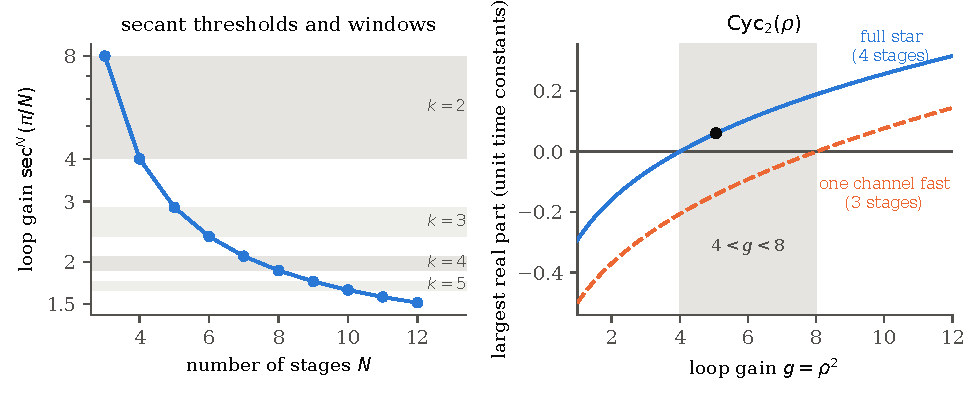
\includegraphics[width=\linewidth]{figures/fig_secant.pdf}
\caption{Left: the secant thresholds $\sec^N(\pi/N)$; for $k$ channels the window of
Theorem~\ref{thm:sharpness} lies between $N=2k$ and $N=2k-1$ stages (shaded for
$k=2,\dots,5$). Right: for $\Cyc_2$, the largest real part at unit time constants of the
full star (a $4$-stage cycle) and of the boundary systems with one fast channel ($3$-stage
cycles), as functions of the loop gain $g=\rho^2$. In the window $4<g<8$ only the star
itself is unstable; the dot marks Example~\ref{ex:cyc2}, $g=81/16$.}
\label{fig:secant}
\end{figure}

\begin{example}[$k=2$]\label{ex:cyc2}
Take $\rho=9/4$, so $g=81/16$ and~\eqref{eq:window} reads $9/8>1$ and $81/128<1$. At unit
time constants the characteristic polynomial of $\Cyc_2(9/4)$ is $(\lambda+1)^4+81/16$,
whose roots are $-1+\tfrac32e^{\pm i\pi/4}$ and $-1+\tfrac32e^{\pm3i\pi/4}$. The first pair
has real part $\tfrac{3\sqrt2}{4}-1\approx0.0607>0$, and the Routh array has two sign
changes. The nine boundary systems are listed in Table~\ref{tab:cyc2}. A slow channel cuts
the cycle. Two fast channels leave a $2$-stage cycle on the core, with matrix
$-I+\rho(\be_0\be_1^\T-\be_1\be_0^\T)$, which is D-stable for every $\rho$. One fast and
one synchronized channel leave a $3$-stage cycle of gain $81/16<8=\sec^3(\pi/3)$. Only the
fully synchronized choice, which is the star itself, is unstable.
\end{example}

\begin{table}[tb]
\centering\small
\caption{Boundary systems of $\Cyc_2(9/4)$; $\sigma=(\sigma(0),\sigma(1))$, loop gain
$g=81/16$. ``Stages'' counts the first-order stages left on the feedback cycle.}\label{tab:cyc2}
\begin{tabular}{@{}lllll@{}}
\toprule
$\sigma$ & reduced model & stages & verdict & reason\\
\midrule
$(\rS,\cdot)$, $(\cdot,\rS)$ & a frozen piece & cycle cut & D-stable & triangular after permutation\\
$(\rF,\rF)$ & both pieces quasi-steady & 2 & D-stable & $2\times2$: trace $<0$, det $>0$\\
$(\rF,\rD)$, $(\rD,\rF)$ & one piece quasi-steady & 3 & D-stable & $g<\sec^3(\pi/3)=8$\\
$(\rD,\rD)$ & the full star & 4 & D-unstable & $g>\sec^4(\pi/4)=4$\\
\bottomrule
\end{tabular}
\end{table}

% =========================================================================
\section{Discussion}\label{sec:discussion}

\paragraph{What the theorems say for reduced models.} Theorem~\ref{thm:localization} says
that every way in which a star can reach or cross the imaginary axis, for some choice of
time constants, is already present, at the same eigenvalue, in a reduced model built by
quasi-steady elimination, freezing and lumping, with at most one lumped pool per interface
(possibly at other core time constants). Theorem~\ref{thm:lifting} says that nothing is lost
in the other direction for strict instability: a reduced model with a growing mode certifies
a growing mode of the full model, at a nearby eigenvalue, when the lumped pools keep their
time constants, the eliminated pieces are fast enough and the frozen pieces slow enough.
Theorem~\ref{thm:sharpness} and Proposition~\ref{prop:lumping} show that the lumped pools
cannot be dropped: in $\Cyc_k$ every reduced model with a quasi-steady or frozen channel is
D-stable, and the instability appears only with all $k$ channels dynamic; and in the example
of Proposition~\ref{prop:lumping} it appears only when two pieces are lumped.

\paragraph{The marginal case.} Corollary~\ref{cor:criterion} decides D-semistability exactly,
but D-stability only in one direction. When all boundary systems are D-semistable and some
are marginal, the star is D-semistable, and it is D-stable exactly when no positive scaling
of it has an eigenvalue on the imaginary axis. Theorem~\ref{thm:localization} transfers such
eigenvalues to boundary systems but not back, and Proposition~\ref{prop:gap} shows that the
transfer back can fail. For one coordinate channel with positive loads, a D-stable core and
$n\ge2$, the companion paper~\cite[Lemma~6.1]{companionI2026} closes this gap: the star is
D-stable if and only if $\det(-B_{\sigma\equiv\rF})>0$ and every boundary system with at most
one dynamic piece, other than the purely static $\Bd_{\sigma\equiv\rF}$, is D-stable.
Proposition~\ref{prop:gap} is an instance, in which the purely static system is the only
marginal one.

\paragraph{Size of the reduction.} The number of boundary choices is $3^m$; by
Remark~\ref{rem:scope}(iii) only the per-channel pairs of fast and synchronized load sums
matter, which reduces the count substantially when loads repeat. For binary-encoded loads,
deciding D-stability of stars is coNP-hard, and deciding D-instability NP-hard, already for
one coordinate channel and a $4\times4$ core with instance-dependent entries of polynomial
bit length~\cite{companionHard2026}. So, unless $\mathrm{P}=\mathrm{NP}$, no procedure
examines boundary systems in time polynomial in the binary input.

\paragraph{Open problems.}
\begin{enumerate}[label=(\arabic*)]
  \item \emph{Coordinate channels.} The channels of $\Cyc_k$ read one coordinate and act on
    another. For coordinate channels, $u_c=v_c=\be_{i_c}$, with positive loads, it is open
    whether two channels can require two synchronized groups.
  \item \emph{The marginal case} for general interfaces: which additional reduced
    information decides D-stability when some boundary systems are marginal?
  \item \emph{Higher-order attachments.} For attachments of higher order the value of a
    module at a fixed eigenvalue ranges over a two-dimensional region rather than an arc,
    and the boundary structure of Minkowski sums of such regions replaces
    Lemma~\ref{lem:sync}.
  \item \emph{Nonlinear dynamics.} The results are linear and spectral; they say nothing
    directly about the nonlinear onset of oscillations.
\end{enumerate}

% =========================================================================
\section{Formal verification}\label{sec:lean}

The results are formally verified in Lean~4 (v4.30.0) with Mathlib at revision
\lean{c5ea00351c28} (the full hash is in the ancillary Lake manifest). The development consists of the modules
\lean{proofs/DStabilityLocalization/*.lean} and the definition file
\lean{proofs/DUnstableCores/DScaling.lean}, which defines positive scalings
(\lean{rightScale}), eigenpairs (\lean{HasEigenpair}) and the predicates \lean{DStable},
\lean{DNonUnstable} (D-semistable) and \lean{DUnstable} exactly as in
Section~\ref{sec:setting}; an eigenpair is a nonzero complex vector $y$ with $(AD)y=zy$.

The root declaration \lean{DStabilityLocalization.localization_and_sharpness} states, for all
finite index types in the universe \lean{Type}: Theorem~\ref{thm:lifting} for arbitrary
loads; Theorem~\ref{thm:localization} and Corollary~\ref{cor:criterion} for nonzero loads;
Theorem~\ref{thm:sharpness} as printed, for every $k=m+2$ (explicit eigenvalue, instability,
D-stability of the boundary systems with fewer than $k$ groups for every $\rho$
satisfying~\eqref{eq:window}, and existence of such $\rho$); Propositions~\ref{prop:gap}
and~\ref{prop:lumping} as printed; and the verdicts of Example~\ref{ex:cyc2}. The lemmas are
declarations on which the root depends, with the statements printed here; in particular
Lemma~\ref{lem:boundary} exhibits the scaling $\diag(q,\tau)^{-1}$, and
Lemmas~\ref{lem:zero} and~\ref{lem:real} keep the core time constants, as in
Remark~\ref{rem:scope}(i). The root depends only on the axioms \lean{propext},
\lean{Classical.choice} and \lean{Quot.sound}; no \lean{sorry}, custom axiom or native
computation is used. Table~\ref{tab:lean} lists the declarations. Remarks and the modelling
reading are not formalized, except Remark~\ref{rem:scope}(iii), which is
\lean{bdSystem_eq_of_loads} in a separate module outside the root. The characteristic
polynomial, roots and Routh array of Example~\ref{ex:cyc2}, the Hurwitz data behind
Table~\ref{tab:cyc2}, the values plotted in the figures, and the source hashes of the
compilation receipt are replayed exactly by the script \lean{check_paper.py}. The Lean
sources, the strict compilation receipt (warnings treated as errors), the replay script and
the two companion manuscripts form the ancillary material.

\begin{table}[tb]
\centering\small
\caption{Lean declarations (namespace \texttt{DStabilityLocalization}).}\label{tab:lean}
\begin{tabular}{@{}>{\raggedright\arraybackslash}p{0.30\linewidth}>{\raggedright\arraybackslash}p{0.64\linewidth}@{}}
\toprule
Result & Declarations\\
\midrule
Definitions~\ref{def:star}, \ref{def:boundary} & \lean{star}, \lean{pencil}, \lean{lagValue}, \lean{Role}, \lean{bdCore}, \lean{bdLoad}, \lean{bdSystem}, \lean{groups}\\
Lemma~\ref{lem:elimination} & \lean{pencil_kernel_of_eigenpair}, \lean{eigenpair_of_pencil_kernel}\\
Lemma~\ref{lem:affine} & \lean{det_sub_smul_vecMulVec}\\
Lemma~\ref{lem:dilation} & \lean{pencil_det_ne_of_large}, \lean{pencil_det_ne_of_norm}\\
Lemma~\ref{lem:arc} & \lean{val}, \lean{val_zero}, \lean{val_one}, \lean{lag_eq_val}, \lean{val_eq_lag}, \lean{norm_val_le_one}, \lean{hasStrictDerivAt_val}\\
Lemma~\ref{lem:sync} & \lean{sync_det}, \lean{sync_det_ne}\\
Lemma~\ref{lem:open} & \lean{open_two_pieces}\\
Lemma~\ref{lem:exit} & \lean{exit_channel}\\
Proposition~\ref{prop:induction} & \lean{localize_all}\\
Lemma~\ref{lem:boundary} & \lean{pencil_boundary}, \lean{boundary_eigenpair}\\
Theorem~\ref{thm:localization}, non-real $z$ & \lean{localization_nonreal}\\
Lemmas~\ref{lem:zero}, \ref{lem:real} & \lean{zero_eigen_static}, \lean{localization_real}\\
Theorem~\ref{thm:localization} & \lean{spectral_localization}\\
Theorem~\ref{thm:lifting} & \lean{dUnstable_of_boundary}, with \lean{hurwitz_zero}, \lean{exists_sphere_ne}\\
Corollary~\ref{cor:criterion} & \lean{dStable_of_boundary}, \lean{dNonUnstable_iff}, \lean{dUnstable_iff}\\
Proposition~\ref{prop:gap} & \lean{gap_star_dStable}, \lean{gap_static_eigenpair}, \lean{marginal_gap}\\
Lemmas~\ref{lem:secant}, \ref{lem:mono} & \lean{secant_inequality}, \lean{cos_pow_strictMono}\\
Theorem~\ref{thm:sharpness} & \lean{cycStar}, \lean{cycEig}, \lean{cyc_star_eigenpair}, \lean{cycEig_re_pos}, \lean{cyc_star_dUnstable}, \lean{cyc_lower_dStable}, \lean{cyc_window}, \lean{sharpness_full}\\
Lemma~\ref{lem:cubic} & \lean{cubic_ne_zero}\\
Proposition~\ref{prop:lumping} & \lean{lump_star_eigenpair}, \lean{lump_lower_dStable}, \lean{lumping_needed}\\
Example~\ref{ex:cyc2}, Table~\ref{tab:cyc2} & \lean{cyc2_example}\\
Root & \lean{localization_and_sharpness}\\
\bottomrule
\end{tabular}
\end{table}

\bibliographystyle{plainurl}
\bibliography{refs}

\end{document}
